\documentclass[a4paper, twocolumn]{jsarticle}
\usepackage[dvipdfm]{graphicx}

\begin{document}

\title{ベンフォードの法則によるフェイクレビュー検出手法の検討}
\author{
  NECO B2 江頭叙那(jonah)
  \\ 親 ks91 
}
\maketitle

\section{はじめに}

ネットショッピングが普及し,多くの人々がオンラインで買い物
をするようになった.商品のレビューはユーザーが購入を検討する際に大きな要因となるが,
企業が金銭を見返りに偽のレビューを書かせるフェイクレビューが問題になっている.

\section{目的}
ベンフォードの法則を応用した素性を利用して,既存方式よりも
少ない情報から,商品にフェイクレビューが含まれているかどうか
を検出することを目指す.

\section{ベンフォードの法則の概要}
ベンフォードの法則とは,電気料金の請求書,住所の番地,
株価,人口,革の長さ,物理・数学定数などの自然界に現れる
数値集合の各数値における最上位桁の数値の出現確率には偏り
があるという法則である.この分布から大きく離れている場合,
何らかの人手による操作などが行われた可能性がある.\cite{benford}

\section{仮説}
偽のレビューを書くレビュアーは実際に商品を使っておらず,さらに
報酬を得るために短期間で多くのレビューを書く必要があるため,他のレビューを参考に
似た文章を書くケースが多いのではないかと考える.そのため,フェイクレビューを含んでいない
商品と比べて,使用される文字の頻度の分布が異なるのではないかと考えた.


\section{既存方式}
Amazonのフェイクレビューを見抜くサクラチェッカー \cite{sakura}
では,価格・製品,レビュー分布やショップレビューなど
計8項目の情報を,独自のロジックや機械学習を用いて分析
している.

\section{既存方式の課題}
サクラチェッカーではAmazonのレビューしか判定する
ことができず,他サイトのレビュー判定ができない.
また,分析項目が多く他サイトに応用しづらい点が
課題である.

\section{提案方式}
1.サクラチェッカーでサクラ度が20\%以下の商品を
安全な商品,80\%以上の商品を危険な商品とし,
2グループそれぞれ200商品のレビューをSeleniumによって
取得する.\cite{amazon}
\\2.取得したレビューの文字の出現頻度
をカウントし,頻度の最上位桁の割合を計算する.
\\3.安全な商品と危険な商品のグループで,最上位桁
の分布がどのように異なるかを分析する.
\\4.分析結果をもとに商品にフェイクレビューが
含まれているかどうかを判定する

\section{結果}
サクラチェッカーによる安全な商品と危険な商品のレビューを
それぞれ200商品ずつ取得し,出現する文字の頻度の最上位桁を
取得した結果が以下のグラフである.\\

\begin{figure}[htbp]
  \begin{center}
    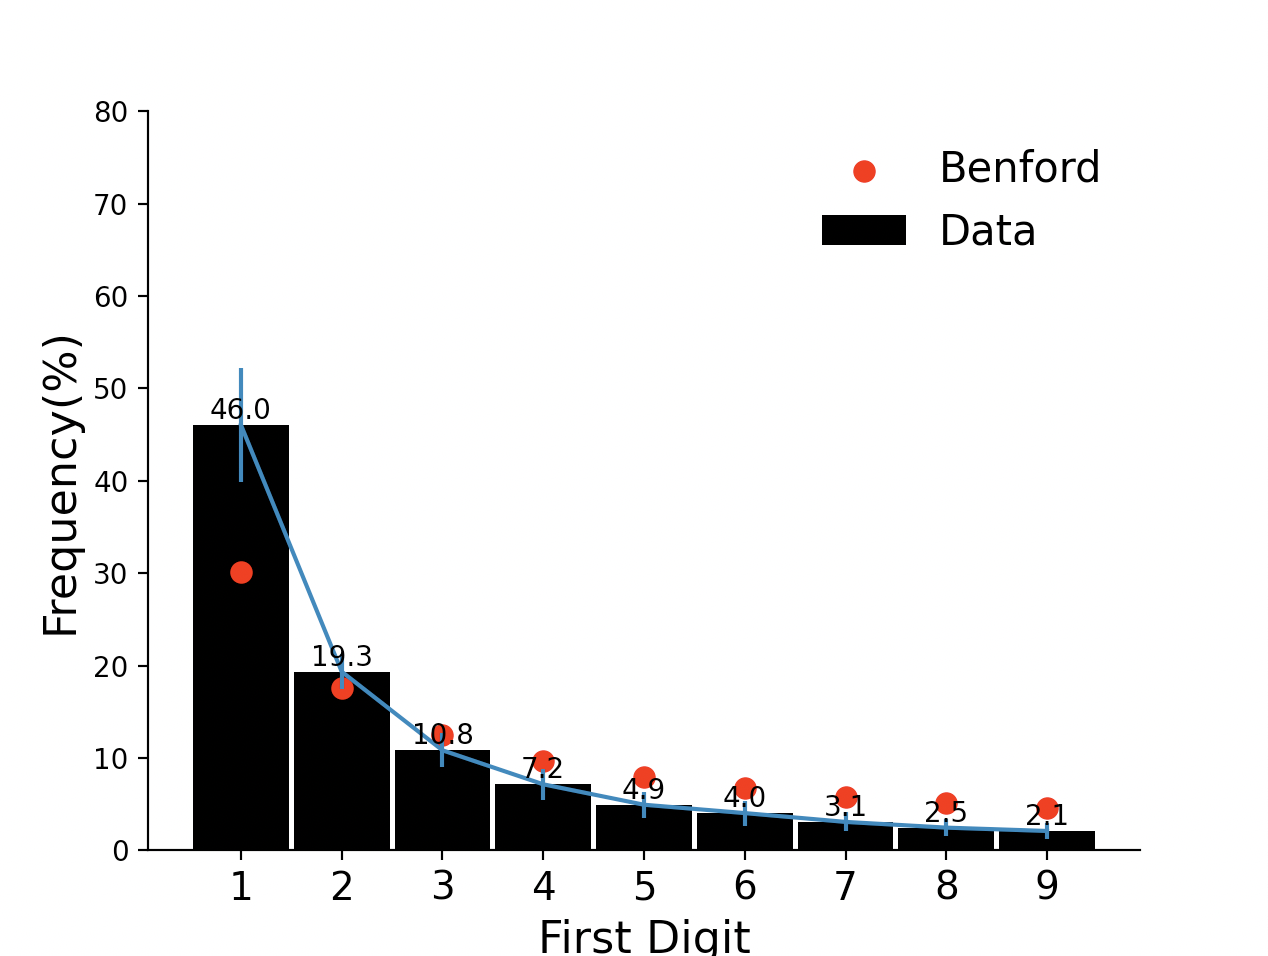
\includegraphics[width=7cm]{./bad_result.png}
    \caption{危険な商品の文字頻度の分布}
    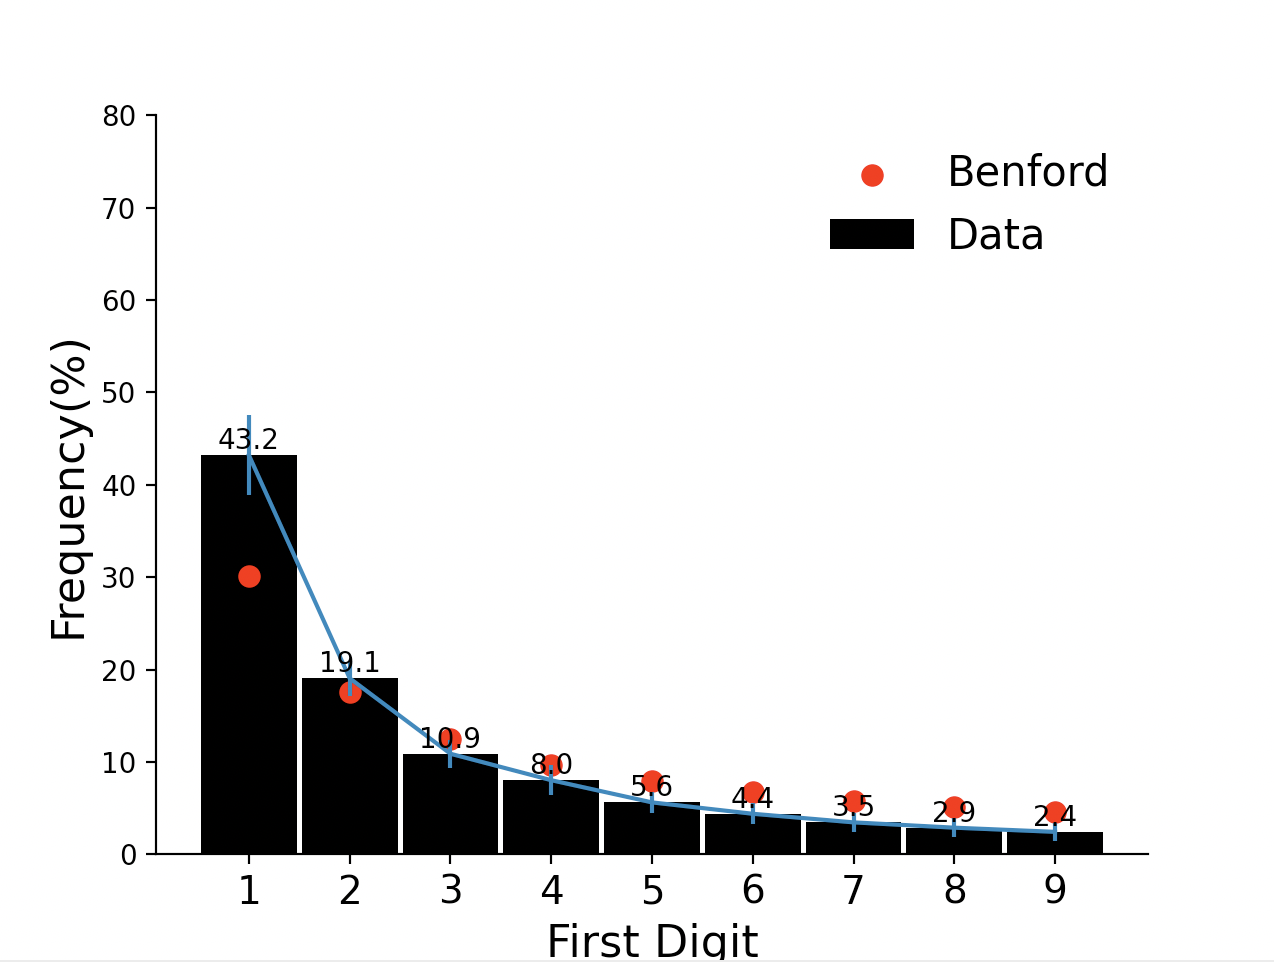
\includegraphics[width=7cm]{./good_result.png}
    \caption{安全な商品の文字頻度の分布}
  \end{center}
\end{figure}%


1の位において,危険な商品のほうが出現頻度が高く標準偏差も大きかったが,
差は僅かであった.そのため,レビューの文字出現頻度から
フェイクレビューが含まれるかを判定することはできなかった.
また,janomeによる形態素解析によって単語に分解し,単語の出現
頻度を分析しても,2つの商品グループに僅かな差しか認められなかった.

\section{考察}
安全な商品と危険な商品の文字の出現頻度の最上位桁の割合
に差がほとんどなかった理由は以下の3つであると考えた.

\begin{enumerate}
  \item フェイクレビュアーが他のレビューを参考に似た文を書いているという仮説が正しくなかった.
  \item 似た文章が多い場合に,文字の分布が異なるのかどうかという検証をしていなかった.
  \item 商品あたりのレビューが少ない場合に,頻度が偏ってしまった.
\end{enumerate}


\section{今後の展望}
ベンフォードの法則を用いてレビューのみからフェイクレビューを検出することは
困難であるとわかった.今後は機械学習の学習を進めて様々な観点からのフェイクレビュー検出を
検討していきたい.

\begin{thebibliography}{99}
  \bibitem{benford} ベンフォードの法則 \\ https://ja.wikipedia.org/wiki/ベンフォードの法則/ (参照 2021/1/27)
  \bibitem{sakura} サクラチェッカー \\ https://sakura-checker.jp/ (参照 2021/1/27)
  \bibitem{vaughan} Lee Vaughan, 高島亮祐訳, ``実用的でないPythonプログラミング'', 第1版, 共立出版(2020)
  \bibitem{kurauchi} 蔵内 雄貴 他, ``ベンフォードの法則を応用したbotアカウント検出'', 日本電信電話株式会社 NTT サービスエボリューション研究所(2013)
  \bibitem{amazon} ジコログ ``Amazonのスクレイピング対策を攻略する'' \\ https://self-development.info/amazonのスクレイピング対策を攻略する【selenium最強説】/ (参照 2021/1/27)
  \bibitem{janome} うぇぶのきわみ, IkeSei, ``pythonで日本語の記事に登場する単語の出現数を調べる方法'' \\ https://web-kiwami.com/count-words-article-python.html (参照2021/1/27)
\end{thebibliography}

\end{document}